\documentclass[tikz, border=3mm]{standalone}
\usepackage{tikz}
\usetikzlibrary{arrows.meta, positioning, calc} % Added calc

\begin{document}
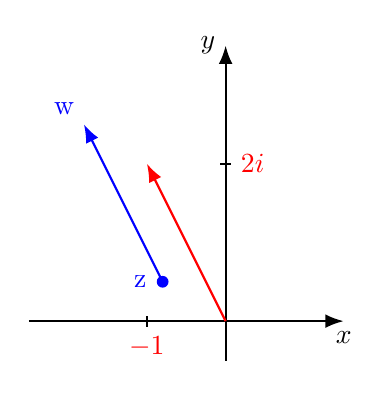
\begin{tikzpicture}[
    >=Latex, % Set default arrow tip style
    tick/.style={thick}, % Style for tick marks
    dot/.style={fill=blue, circle, inner sep=1.5pt} % Style for point z
]

    % Define the red vector displacement (same as its endpoint from origin)
    \coordinate (red_vec_disp) at (-1, 2);
    % Define the start point z (adjust as needed, kept similar to previous estimate)
    \coordinate (z) at (-0.8, 0.5);

    % Calculate the endpoint w by adding the displacement to z
    \coordinate (w) at ($(z) + (red_vec_disp)$);

    % Determine axis limits based on calculated points
    % Need to accommodate origin, red_vec_disp=(-1,2), z=(-0.8,0.5), w approx (-1.8, 2.5)
    \def\xmin{-2.5}
    \def\xmax{1.5}
    \def\ymin{-0.5}
    \def\ymax{3.5}

    % Axes
    \draw[->, thick] (\xmin, 0) -- (\xmax, 0) node[below] {$x$};
    \draw[->, thick] (0, \ymin) -- (0, \ymax) node[left] {$y$};

    % Ticks and Labels
    \draw[tick] (-2pt, 2) -- (2pt, 2); % Tick at y=2
    \node[red, right=2pt] at (0, 2) {$2i$};

    \draw[tick] (-1, -2pt) -- (-1, 2pt); % Tick at x=-1
    \node[red, below=2pt] at (-1, 0) {$-1$};

    % Red Vector (from origin to (-1, 2))
    \draw[->, thick, red] (0,0) -- (red_vec_disp);

    % Blue Vector and Point z
    % Draw point z indicator and label
    \node[dot, label={[blue] left:z}] at (z) {};

    % Draw blue vector w (from z to calculated w)
    \draw[->, thick, blue] (z) -- (w);
    \node[blue, above left] at (w) {w}; % Label endpoint w

\end{tikzpicture}
\end{document}